
\subsubsection{模糊测试框架}
模糊测试(fuzzing)作为一种基于缺陷注入的自动化软件漏洞挖掘技术,是现在最有效的
漏洞挖掘技术。模糊测试向目标应用程序生成大量的正常和异常输入,并通过将生成的输入
提供给目标应用程序并监视执行状态来检测异常。与其他技术相比,模糊化易于部署,具有
良好的可扩展性和适用性,无论是否使用源代码,都可以执行。同时,由于模糊测试在代码
运行时进行监测,所以其具有较高的精度。

具体而言,模糊测试的工作过程包括四个主要阶段:测试样例生成阶段、测试样例运行阶
段、程序执行状态监控和异常分析阶段。模糊测试主要过程如图X所示。
\begin{figure}[ht]
	\centering
	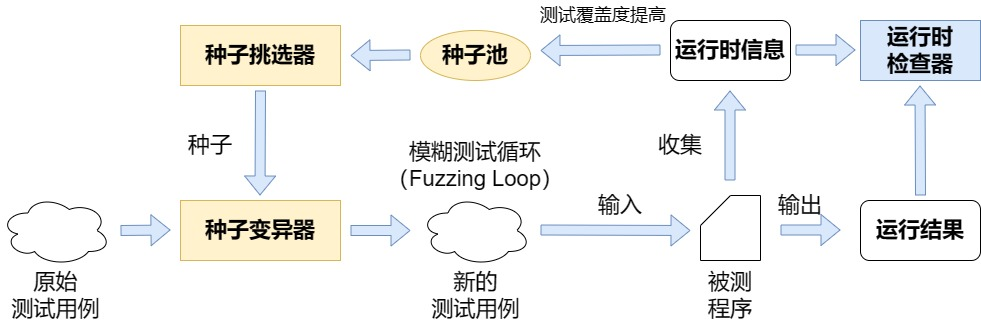
\includegraphics[height=4cm, width=13cm]{fuzzing.jpg}
	\caption{Example of an image}
	\label{fig:fuzzing}
\end{figure}

模糊测试从生成测试用例开始,其生成的测试用例的质量直接影响模糊测试效果。其测试样
例一方面应满足测试程序对输入格式的要求,另一方面输入数据需要包含足够的异常数据,
以便这些输入在被程序处理时很可能导致程序失败或崩溃。根据目标程序的不同,输入可以
是具有不同文件格式的文件、网络通信数据、具有特定特征的可执行二进制文件等。如何生
成具有足够“破坏性”的测试用例是模糊器面临的一个主要挑战。一般来说,在现有的模糊器
中使用两种生成器,即基于生成的生成器和基于突变的生成器。

在前一阶段生成测试样例后,这些测试样例会被送入目标程序。模糊测试工具会自动启动并
结束目标程序的进程,并驱动目标程序的测试样例处理过程。在执行之前,分析人员可以配
置目标程序的启动和结束方式,并预定义参数和环境变量。通常,模糊测试过程会在预定义
的超时时停止,或是在程序执行挂起或崩溃时停止。

模糊测试工具在目标程序执行过程中监控执行情况,期待发现异常和崩溃。常用的异常监控
方法包括对特定系统信号、崩溃以及其他违规行为的监控。对于没有直观程序异常行为的违
规情况,可以使用许多工具,包括AddressSanitizer(Serebryany等,2012
年)、DataFlowsanitizer(The Clang Team,2017a)、ThreadSanitizer(Serebryany和
Iskhodzhanov,2009年)、LeakSanitizer(The Clang Team,2017b)等。当捕获到违规行
为时,模糊测试工具会存储相应的测试样例,以供后续重放和分析。在分析阶段,分析人员
尝试确定捕获的违规行为的位置和根本原因。分析过程通常借助调试器完成,比如
GDB、windbg,或其他二进制分析工具,如IDA Pro、OllyDbg等。二进制插桩工具,如Pin
等,也可以用来监控收集到的测试样例的确切执行状态,例如线程信息、指令、寄存器信息
等。自动崩溃分析是另一个重要的研究领域。

在执行完上述四个阶段之后,将根据程序反馈即代码覆盖率是否提升来判断种子是否有趣,
有趣的种子将被加入种子池中进行后续变异,进而形成新的测试样例重新输入待测程序。具
体而言,判断种子是否有趣的原则为选取开销小,作用大的种子,即如果两个种子可以得到
相同的代码逻辑覆盖情况,则保留文件较小的种子;如果两个种子可以得到相同的代码逻辑
覆盖情况,则选择耗时较小的。

根据程序源代码的依赖程度和程序分析的程度,模糊测试工具可以分为白盒、灰盒和黑盒。
白盒模糊测试假定能够访问程序的源代码,因此可以通过对源代码的分析以及测试用例如何
影响程序运行状态来收集更多信息。黑盒模糊测试在没有任何关于目标程序内部的知识的情
况下进行模糊测试。灰盒模糊测试也不需要源代码,通过程序分析来获得目标程序的内部信
息。

具体而言,白盒模糊测试是一种利用程序的内部结构和实现细节来生成测试用例的测试方
法。不同于黑盒模糊测试仅基于输入和输出进行测试,白盒模糊测试要求测试者对程序的内
部结构有深入了解。通过分析程序的源代码,白盒模糊测试使用符号执行和约束求解技术来
自动生成能够覆盖程序不同路径的输入数据,目标是深入程序内部逻辑以发现深层次的安全
漏洞和错误。

白盒模糊测试的一个核心特点是它的能力来处理高度结构化的输入,如编译器和解释器等应
用程序。这些应用程序按阶段处理输入,例如词法分析、解析和求值。白盒模糊测试结合了
静态分析和动态测试生成的方法,通过执行程序的符号执行并在此过程中生成和求解约束,
以自动化的方式生成测试输入。

白盒模糊测试在自动化测试生成、测试用例的执行以及测试结果的分析方面的广泛应用。这
包括但不限于利用程序分析技术优化测试过程、缩小输入空间、提高测试的自动化水平等。
白盒模糊测试通过这些技术手段实现了对复杂软件系统的有效测试,能够更加准确地发现并
定位软件中的安全漏洞和错误。

\subsubsection{ASan}

[5]在模糊测试阶段自动分析运行时信息和输出结果时,程序会进行缺陷检测,而ASan(即
AddressSanitizer)是一种专为C和C++等编程语言设计的快速的内存错误检测工具,可以有
效地识别内存访问错误,包括堆、栈和全局变量的越界访问以及使用已释放堆内存
(use-after-free)的错误。具体而言,它采用了一种特殊的内存分配器和足够简单到可以
在任何编译器、二进制转换系统甚至在硬件中实现的代码插桩技术。ASan在不牺牲全面性的
情况下实现了高效率,其平均运行速度减慢仅为73\%,但它能够准确地在发生错误时立即检
测到错误。

ASan由两部分组成:一个插桩模块和一个运行时库。插桩模块修改代码以检查每次内存访问
的影子状态,并在栈和全局对象周围创建有毒的红色区域以检测溢出和下溢。当前的实现基
于LLVM编译器基础设施。运行时库替换了malloc、free及相关函数,围绕分配的堆区域创建
有毒的红色区域,延迟已释放的堆区域的重用,并进行错误报告。

从高层次上看,ASan对内存错误检测的方法与基于Valgrind的工具AddrCheck 类似:使用影
子内存记录每个应用程序内存字节是否安全访问,并使用插桩来在每个应用程序加载或存储
时检查影子内存。与之不同的是,ASan使用了更高效的影子映射、更紧凑的影子编码,在检
测堆外还能检测栈和全局变量中的错误,并且比AddrCheck快一个数量级。接下来将描述
ASan如何编码和映射其影子内存、插入其插桩,以及其运行时库如何操作。

\textbf{(一)影子内存}

malloc函数返回的内存地址通常至少对齐到8字节。这导致任何对齐的8字节序列的应用程序
堆内存都处于9种不同状态之一:前k个(0 $\leq$ k $\leq$ 8)字节是可寻址的,而剩下
的8 $-$ k字节则不是。这种状态可以编码成一个影子内存的单字节。

ASan将虚拟地址空间的八分之一专用于其影子内存,并使用一个比例和偏移的直接映射方式
来将应用程序地址翻译成相应的影子地址。给定应用程序内存地址Addr,影子字节的地址计
算为(Addr$>>$3)+Offset。如果$Max-1$是虚拟地址空间中的最大有效地址,那么Offset的
值应该选择为从Offset到$Offset+Max/8$的区域在启动时不被占用。在典型的32位Linux或
MacOS系统上,其中虚拟地址空间为0x00000000$-$0xffffffff, ASan使用Offset =
0x20000000 (2的29次方)。在一个具有47个有效地址位的64位系统上,我们使用Offset =
0x0000100000000000 (2的44次方)。在某些情况下(例如,在Linux上使用-fPIE/-pie编译
器标志),可以使用零偏移来进一步简化插桩。
\begin{figure}[ht]
	\centering
	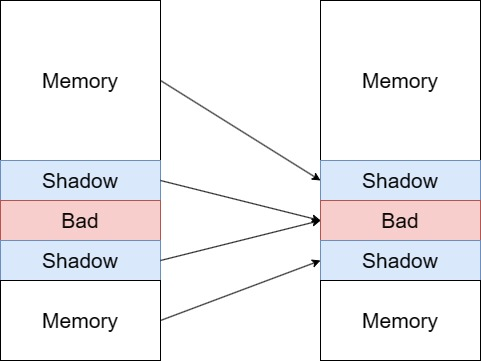
\includegraphics[height=7cm, width=10cm]{shadow.jpg}
	\caption{影子内存地址布局}
	\label{fig:shadow}
\end{figure}

图X展示了地址空间布局。应用程序内存被分为两部分(低和高),它们映射到相应的影子
区域。将影子映射应用于影子区域中的地址会给我们在“坏”区域的地址,该区域通过页面保
护标记为不可访问。

我们对每个影子字节使用以下编码:0意味着相应的应用程序内存区域的所有8字节都是可寻
址的;k(1 $\leq$ k$\leq$ 7)意味着前k个字节是可寻址的;任何负值表示整个8字节字
是不可寻址的。我们使用不同的负值来区分不同种类的不可寻址内存(堆红区、栈红区、全
局红区、释放的内存)。这种影子映射可以概括为形式(Addr$>>$Scale)+Offset,其中
Scale是1...7之一。当Scale=N时,影子内存占据虚拟地址空间的$1/2^N$,红区(以及
malloc对齐)的最小尺寸是$2^N$字节。每个影子字节描述了$2^N$字节的状态,并编码$2^N
+1$不同的值。更大的Scale值需要较少的影子内存但更大的红区来满足对齐要求。Scale值
大于3需要对8字节访问进行更复杂的插桩,但为可能无法放弃其地址空间连续八分之一的应
用程序提供了更多的灵活性。

\textbf{(二)插桩模块}

当对一个8字节的内存访问进行插桩时,AddressSanitizer计算相应影子字节的地址,加载
该字节,并检查它是否为零:

\begin{lstlisting}[language=C++]
ShadowAddr = (Addr >> 3) + Offset;
if (*ShadowAddr != 0)
ReportAndCrash(Addr);
\end{lstlisting}

当对1字节、2字节或4字节的访问进行插桩时,插桩过程会稍微复杂:如果影子值是正数
(即,8字节词中的前k个字节是可寻址的),我们需要将地址的最后3位与k进行比较。

\begin{lstlisting}[language=C++]
ShadowAddr = (Addr >> 3) + Offset;
k = *ShadowAddr;
if (k != 0 && ((Addr & 7) + AccessSize > k))
  ReportAndCrash(Addr);
\end{lstlisting}

在这两种情况下,插桩仅在原始代码的每次内存访问中插入一个内存读取。我们假设一个N
字节的访问是对齐到N的。ASan可能会错过由于未对齐访问引起的错误。

ASan的插桩阶段处在LLVM优化管道的最末端。这样我们只对那些经过LLVM优化器的所有标量
和循环优化后仍然存在的内存访问进行插桩。例如,通过LLVM优化掉的本地栈对象的内存访
问将不会被插桩。同时,我们不需要对LLVM代码生成器生成的内存访问进行插桩(例如,寄
存器溢出)。

\textbf{(三)运行库}

运行时库的主要目的是管理影子内存。在应用程序启动时,整个影子区域都会被映射,以便
程序的其他部分无法使用它。影子内存的坏段被保护起来。在Linux上,影子区域在启动时
总是未被占用的,因此内存映射总是成功的。在MacOS上,我们需要禁用地址空间布局随机
化(ASLR)。我们的初步实验表明,相同的影子内存布局也适用于Windows。

malloc和free函数被替换为特殊的实现。malloc函数在返回的区域周围分配额外的内存,即
红色区域(redzone)。红色区域被标记为不可寻址或“有毒”的。红色区域越大,将能检测
到的溢出或下溢也越大。

分配器内的内存区域被组织为一个自由列表数组,对应于一系列对象大小。当与请求的对象
大小相对应的自由列表为空时,将从操作系统(例如,使用mmap)分配一大组带有红色区域
的内存区域。对于n个区域,我们分配n + 1个红区,使得一个区域的右红区通常是另一个区
域的左红区:

\begin{figure}[ht]
	\centering
	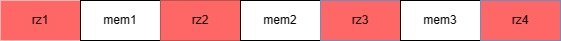
\includegraphics[height=1cm, width=15cm]{rz.jpg}
	\caption{红区分布}
	\label{fig:rz}
\end{figure}

左红区域用于存储分配器的内部数据(如分配大小、线程ID等);因此,堆红区的最小尺寸
当前为32字节。这些内部数据不会因为缓冲区下溢而被破坏,因为这种下溢会在实际存储之
前立即被检测到(如果下溢发生在被插桩的代码中)。

free函数将整个内存区域标记为有毒,并将其放入隔离区,以便这个区域在短期内不会被
malloc重新分配。目前,隔离区被实现为一个FIFO队列,随时持有固定数量的内存。

默认情况下,malloc和free记录当前的调用堆栈,以提供更多信息的错误报告。malloc调用
堆栈存储在左红区域(红区越大,可以存储的帧数就越多),而free调用堆栈存储在内存区
域的开始处。

为了检测对全局变量和栈对象的越界访问,ASan必须在这些对象周围创建有毒的红区。对于
全局变量,红区在编译时创建,并且红区的地址在应用程序启动时传递给运行时库。运行时
库函数将红区标记为有毒,并记录地址以供进一步的错误报告。

对于栈对象,红区在运行时创建并标记为有毒。目前,使用了32字节的红区(加上最多31字
节用于对齐)。例如,给定一个程序:

\begin{lstlisting}[language=C++]
void foo() {
	char a[10];
	<function body>
}
\end{lstlisting}

转换后的代码将类似于:

为了检测对栈对象的越界访问,AddressSanitizer对原有的函数foo进行了转换,增加了红
区(redzones)来围绕数组arr。这些红区在运行时被标记为“有毒”的,用于捕获任何对这
些区域的非法访问。下面是转换后的代码示例:

\begin{lstlisting}[language=C++]
void foo() {
	char rz1[32]; // 前红区
	char arr[10]; // 原始数组
	char rz2[54]; // 后红区,大小为32-10+32
	unsigned *shadow =
	(unsigned*)(((long)rz1>>8)+Offset);
	// 标记红区和数组周围为有毒
	shadow[0] = 0xffffffff; // rz1
	shadow[1] = 0xffff0200; // arr 和 rz2
	shadow[2] = 0xffffffff; // rz2

	// 函数体
	// 解毒所有区域
	shadow[0] = shadow[1] = shadow[2] = 0;
}
\end{lstlisting}

同时,ASan是线程安全的。影子内存只在相应的应用程序内存不可访问时被修改(在malloc
或free内部、在创建或销毁栈帧期间、在模块初始化期间)。所有其他对影子内存的访问都
是读操作。malloc和free函数使用线程局部缓存来避免每次调用都进行锁定(正如大多数现
代malloc实现所做的)。如果原始程序在内存访问和该内存的删除之间存在竞态,ASan有时
可能将其检测为使用后释放错误,但不能保证总能检测到。每次malloc和free的线程ID都被
记录,并在错误消息中与线程创建的调用栈一起报告。

\subsubsection{基于覆盖率的遗传算法}

基于代码覆盖率的遗传算法是一种将遗传算法原理应用于软件测试的方法,特别是在模糊测
试中,目的是通过优化测试用例来提高代码覆盖率,从而提升软件测试的全面性和效率。遗
传算法是受自然选择原理启发的优化技术,通过模拟生物进化过程中的选择、交叉(杂交)
和变异操作,来在解空间中搜索最优解。

具体而言,在进行模糊测试的过程中,程序通过代码覆盖率的高低来判断种子是否有趣。代
码覆盖率是一种简单的动态分析方法,常用于衡量测试的全面性。它通过将源代码分割成具
有一定粒度的“块”并追踪在运行时遇到了哪些块来实现。有时,还会记录在测试中遇到某个
特定块的次数。测量的覆盖率的粒度可以有所不同,并且存在多个定义来命名不同粒度,但
三种常用的定义包括块覆盖率、决策覆盖率和条件覆盖率。块覆盖率:在块覆盖率中,一个
块是指没有if语句或其他控制语句将执行从块中引导出去的代码片段。在运行时计算这些块
的覆盖率。决策覆盖率:决策覆盖率寻找应用程序做出决策的地方,主要是if语句,然后分
析所有可能的决策被覆盖得有多好。条件覆盖率:条件覆盖率也寻找if语句,并尝试追踪这
些分支中所有不同的布尔值是否已经被测试过。然而,如果应用程序的if语句包含多个条件
进行检查,条件覆盖率并不保证决策覆盖率。

基于代码覆盖率的遗传算法首先定义一个适应度函数来衡量测试用例的优劣,这里的适应度
函数即代码覆盖率。算法从一组测试用例开始,构成了初始种群。通过运行这些测试用例并
根据运行信息得到它们的代码覆盖率,以此来评估种群中每个个体的适应度。并将产生的适
应度高的新测试用例替换种群中适应度较低的测试用例。重复上述步骤,直到达到预定的迭
代次数或代码覆盖率达到预期水平。

基于代码覆盖率的遗传算法在模糊测试中起着非常重要的作用,它可以自动化地生成能够触
发新路径的输入,为软件安全和质量提供了一个强大的工具。通过不断地迭代和优化,这种
方法能够有效地提升测试的深度和广度,帮助开发识别和修复软件中的漏洞。

